\chapter{The mechanical design}
\label{sec:mechanicaldesign}
\textit{\textbf{Chapter abstract:} A mechanical concept to design is explained in detail to best match the requirements of a measurement device. These requirements were set to be; measure pressure on multiple points both longitudinal and latitudinal along the running phase of a cross-country ski$^1$, repeatable results from measurements$^2$, detecting start and end of the camber pocket for gripping wax$^3$, detect the difference between a warm and cold cross-country ski$^4$ and detecting twisting in the cross-country ski structure$^5$. A mechanical system was designed and manufactured with a linear weight system and sensor pockets to conduct objective testing of classical cross-country skis.}

\section{Initial phase}
\label{sec:initial}
The initial concept phase of designing and manufacturing a mechanical system focused on establishing properties the system should possess. It was first and foremost important to collect pressure data along the longitudinal and latitudinal lengths of a cross-country ski. On points discussed in Section \ref{sec:background} concerning pressure distribution, a mechanical system would need to hold sensors underneath the ski on multiple points. 
Further development on the idea based of a research project led by Ole Marius Rindal and Jacob Norenberg (Figure \ref{fig:earlyprototype})(Rindal 2017, \textit{personal communication}, December), led to the first concept of mechanical design for this thesis. The properties of the prototype were; collecting the measurements of the pressure on multiple points along the ski$^1$, repeatable measurements with low variance$^2$, detecting the start and end of the camber pocket$^3$, detect differences in a wide range of skis$^4$, and detecting deflection and twisting in the structure of a ski under load$^5$.

\begin{figure*}[!b]
    \centering
    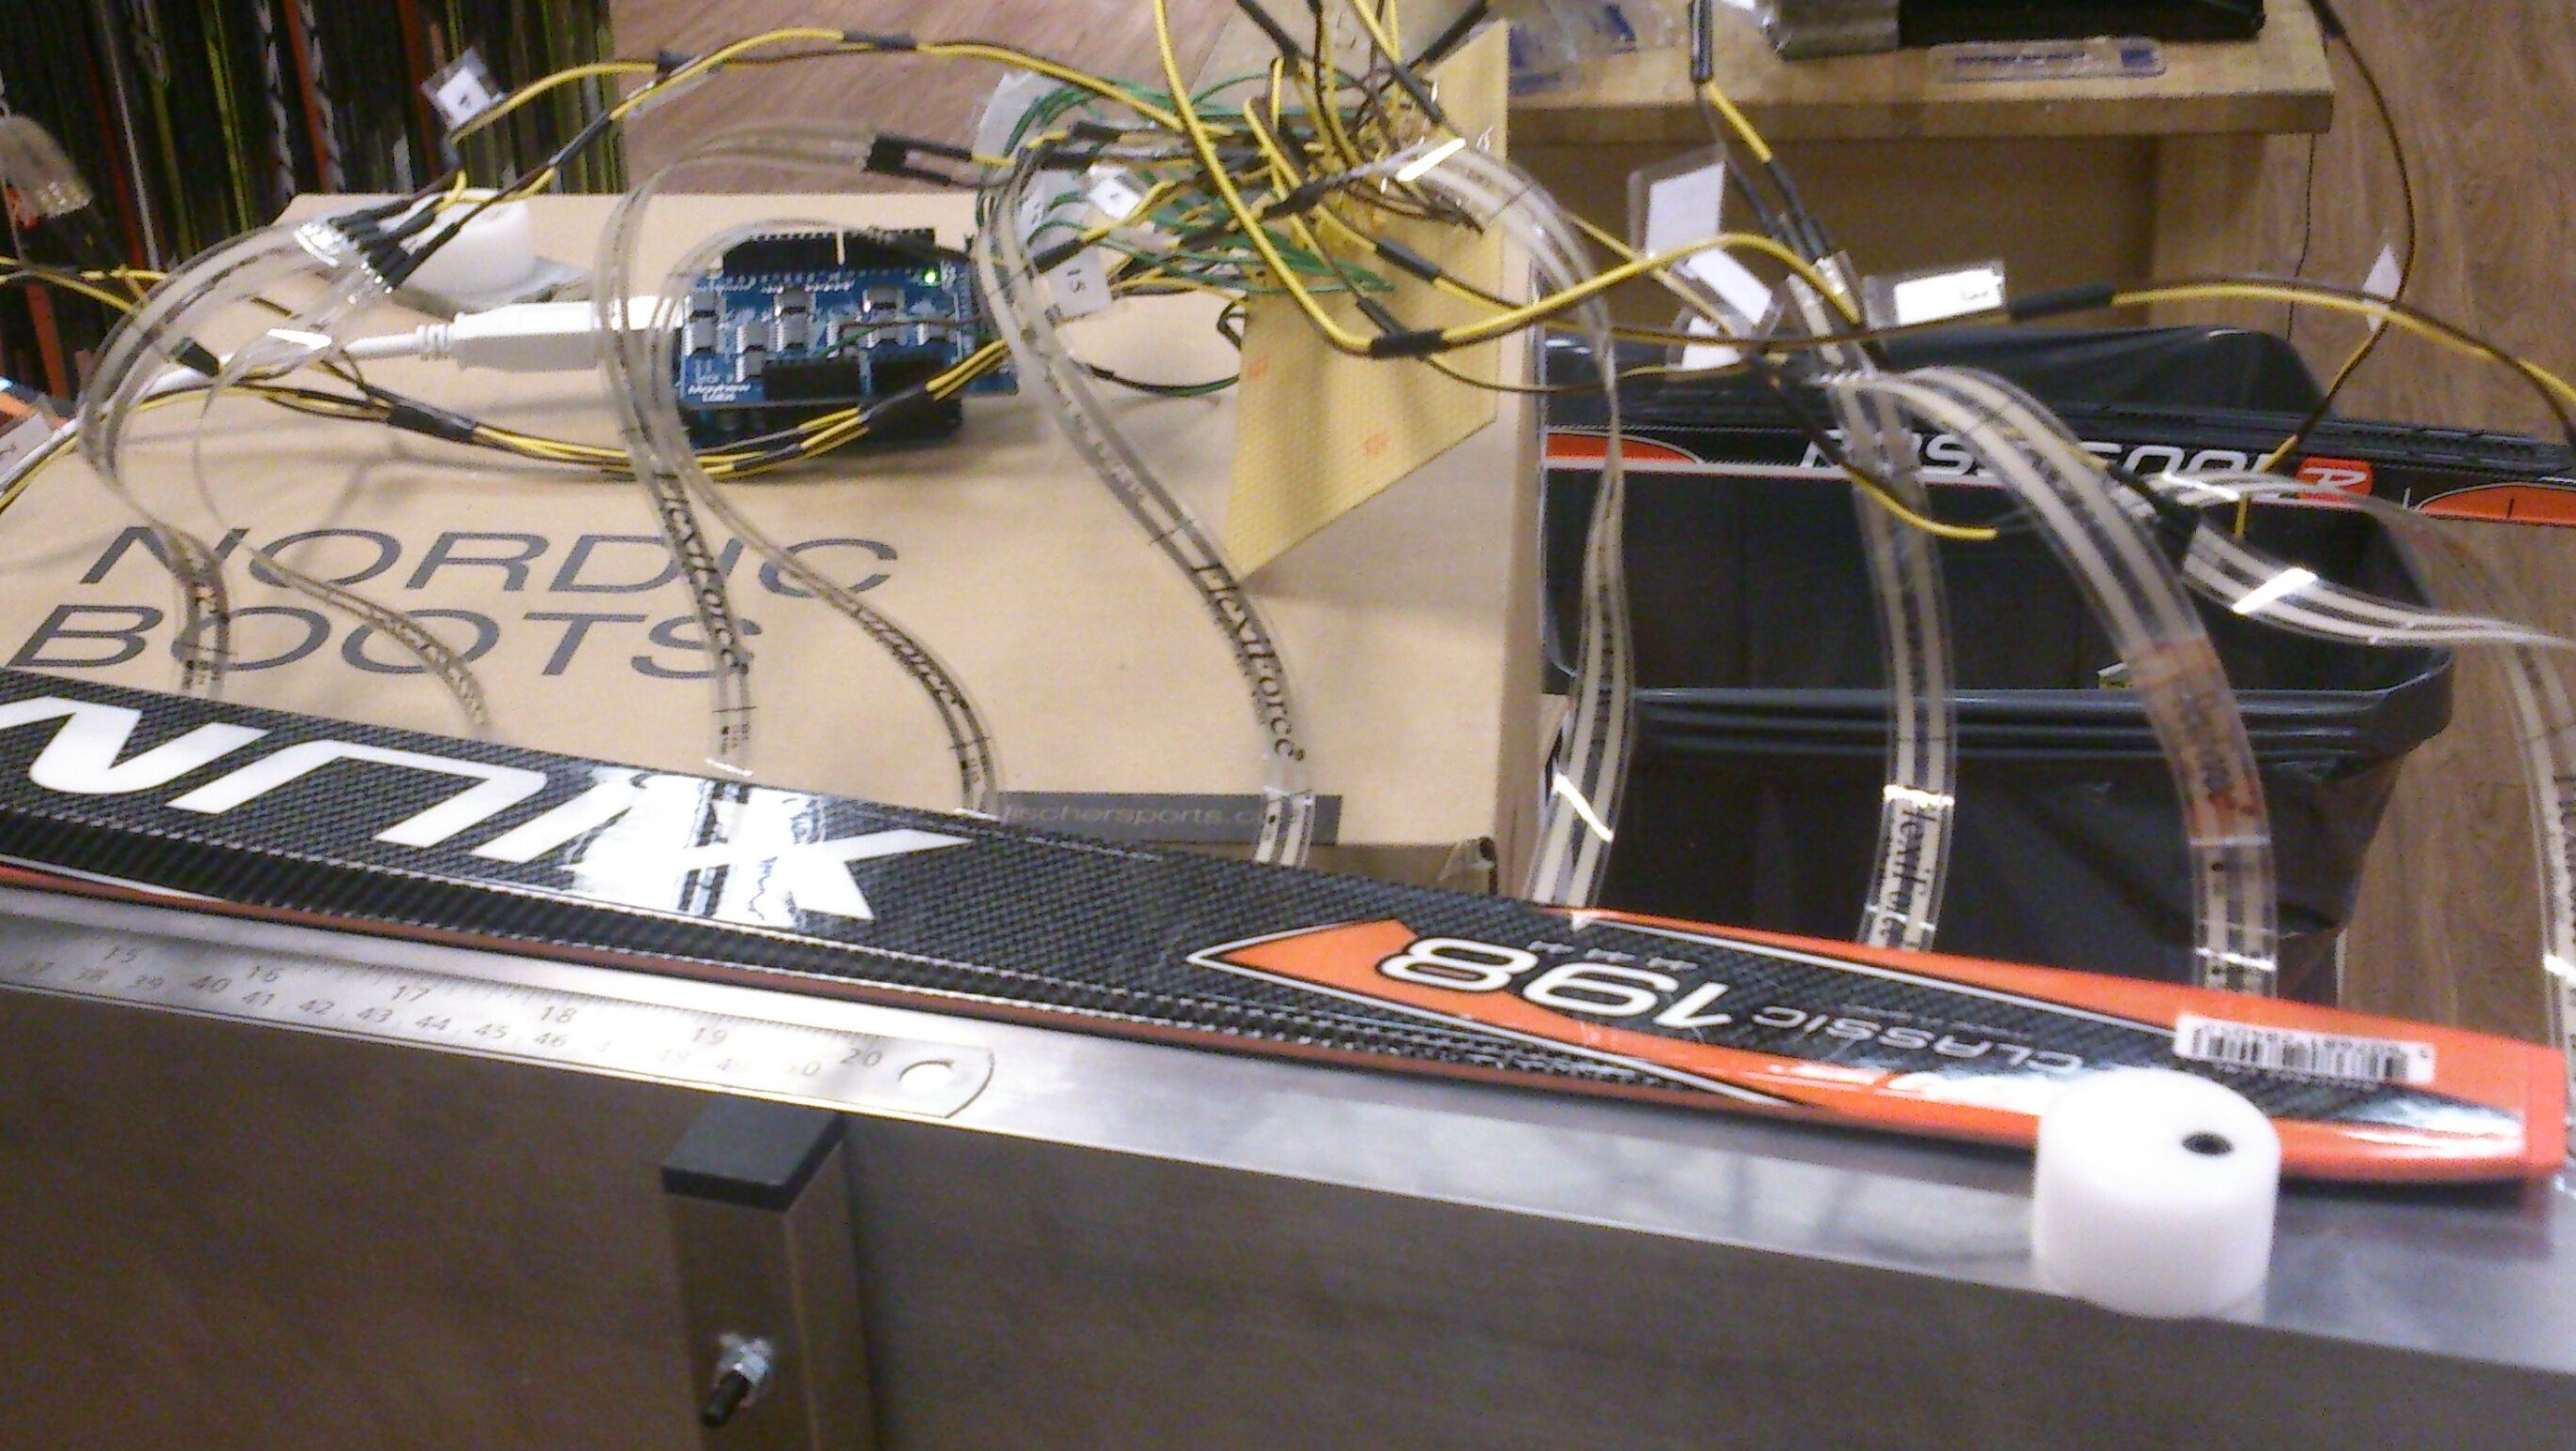
\includegraphics[scale=0.1415]{figures/prototype2.jpeg}
    \caption{Photo of student research project led by Ole Marius Rindal and Jacob Norenberg}
    \label{fig:earlyprototype}
\end{figure*}

\section{Concept 1}
\label{sec:concept1}
The first sketch consisted of a polymethyl methacrylate plate (plexiglass) as a top and bottom surface, enveloping the sensors. The top plate had holes drilled out directly above the sensors, working as a guide for a piston to transfer weight from the ski to the sensor (Figure \ref{fig:earlyconcept}). Enveloping the sensors between two plates, would result in accurate placement of the sensors and locking it in position to avoid movement of the sensor.

\begin{figure}[!htb]
   \begin{minipage}{0.44\textwidth}
     \centering
     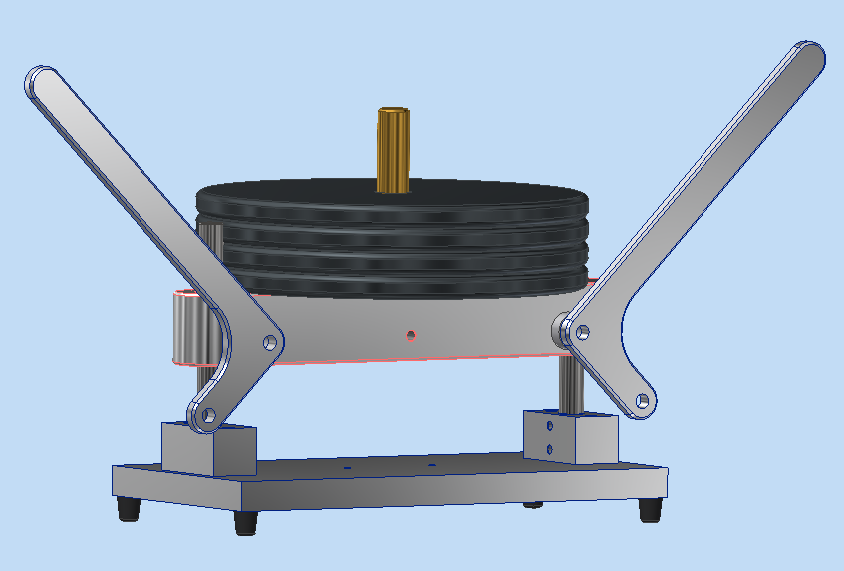
\includegraphics[width=0.9\linewidth]{figures/linearpress2.png}
     \caption{Early concept on sensor placement and structure, hand drawn}
     \label{fig:drawnconcept}
   \end{minipage}\hfill
   \begin{minipage}{0.44\textwidth}
     \centering
     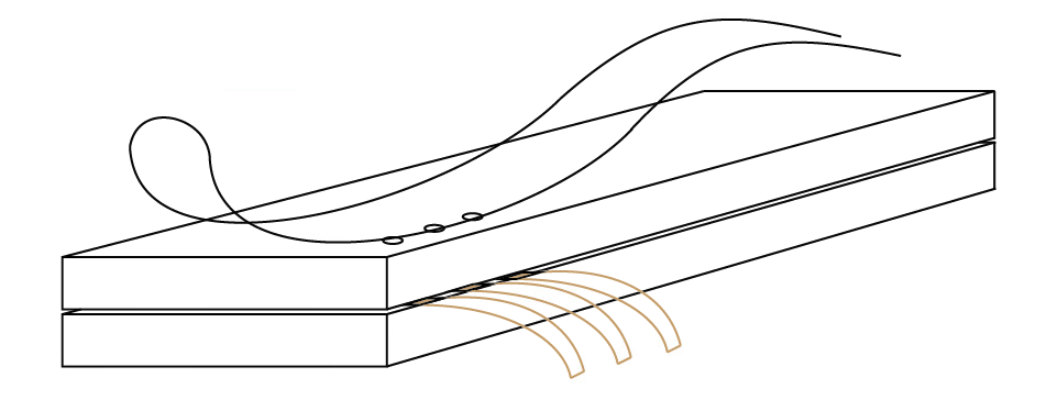
\includegraphics[width=0.9\linewidth]{figures/earlyconcept.png}
     \caption{Early concept on sensor placement and structure, computer drawn}
    \label{fig:earlyconcept}
   \end{minipage}
\end{figure}

\section{Concept 2}
\label{sec:concept2}
To be able to apply force on vertically down on cross-country skis, and calibration of the sensors, one would need a digital weight press or manual weights. During discovery on possible ways of applying weights to the system, there were no cheap alternatives. Reaching out to other sources was necessary.
After consulting with the Instrument Laboratory (I-Lab) at University of Oslo, Department of Physics, we concluded that the bottom surface had to be more rigid than plastic and would need to withstand bending when applying force. The polymethyl methacrylate plates from concept one were not suited for this task, changing the choice of material to aluminum.
I-Lab proposed a solution for applying weight on the ski linearly with a linear weight guide (Figure \ref{fig:linearpress}). The linear guide on its own would not be placing the weight accurately on the ski. A 3D-modelled version of the sketch was drawn with the idea of using aluminum for the whole frame, giving the bench more stability and making it stiffer. The 3D-modelled sketch (Figure \ref{fig:3d-modelledsketch} and \ref{fig:3d-modelledsketch-front}) was drawn in AutoDesk Fusion 360 to visualize the concept of the mechanical design. It became clear that the sensors would need pockets to be placed in the bottom plate to avoid squishing between the plates. The squishing would lead to errors in the measurements due to external forces from the plates onto the sensor.
To produce a mechanical system of this magnitude, we needed a specialized computer numerical control (CNC) machine for accurate placement of the sensor pockets and alignment of assembly points for bolts. Further consultation with I-Lab, led to a collaboration where they were able to manufacture the mechanical system with the needed precision, based on the 3d-model from Figure \ref{fig:3d-modelledsketch}.
The most significant changes in concept 2 were the combination of an aluminum frame with a measurement surface and the linear weight guide attached. These three components together came to be the final result of concept 2. With this in mind, additional development was necessary, in terms of functionality, sensor placement, and locking of the binding to hold the cross-country ski.

\begin{figure}[!htb]
   \begin{minipage}{0.485\textwidth}
     \centering
     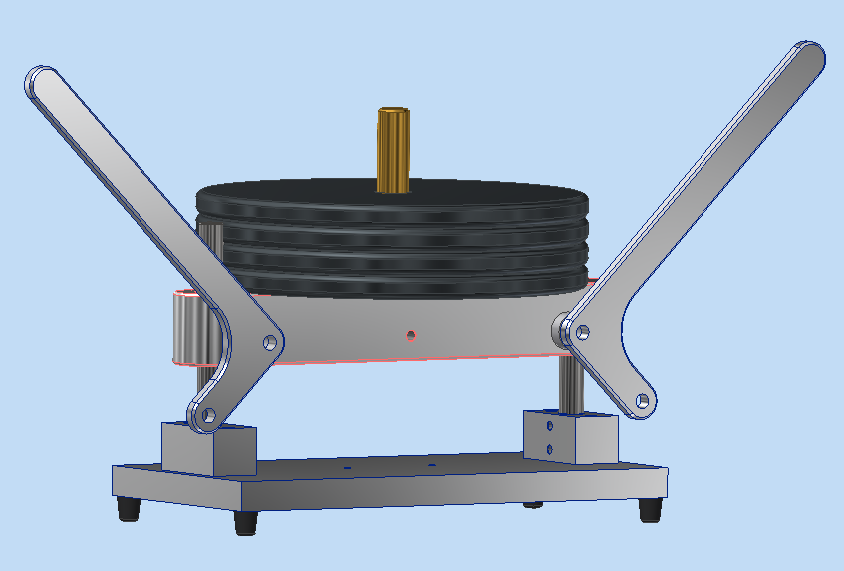
\includegraphics[width=.988\linewidth]{figures/linearpress2.png}
     \caption{Concept for applying forces linearly on a surface.}
     \label{fig:linearpress}
   \end{minipage}\hfill
   \begin{minipage}{0.485\textwidth}
     \centering
     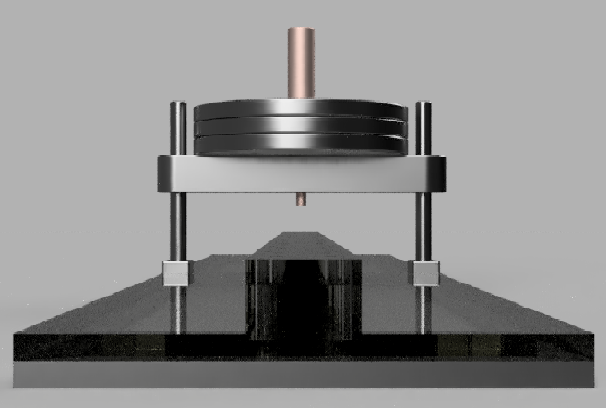
\includegraphics[width=.985\linewidth]{figures/3dsketch_front2.png}
     \caption{3D-model of concept 2, Front side}
     \label{fig:3d-modelledsketch-front}
   \end{minipage}
\end{figure}
\begin{figure*}
    \centering
    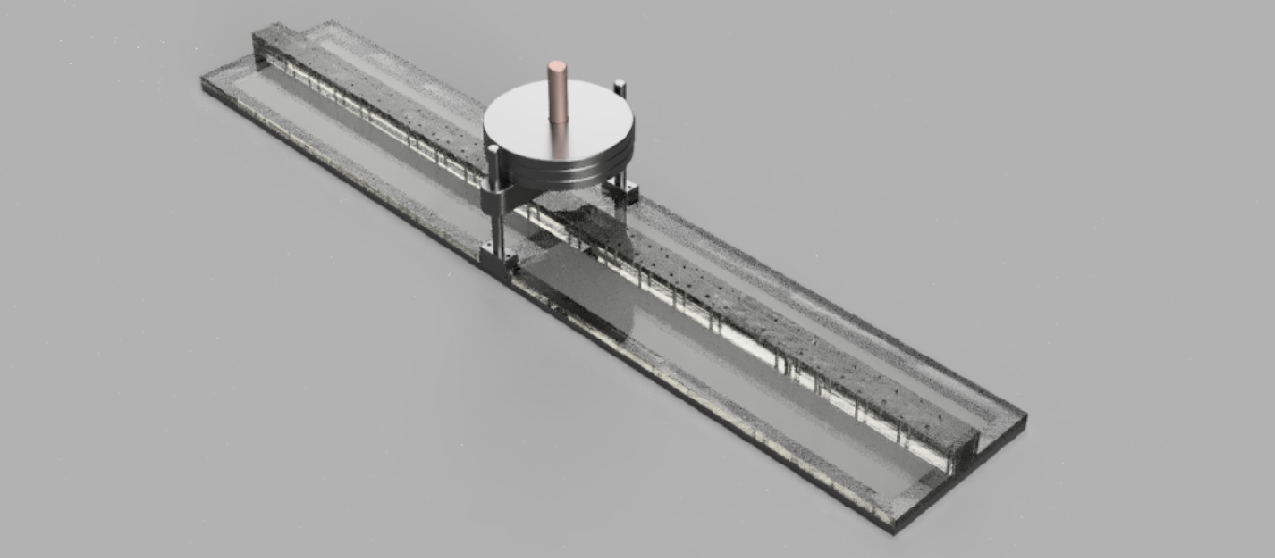
\includegraphics[scale=0.406]{figures/3dmodelledconcept.png}
    \caption{3D-model of concept 2}
    \label{fig:3d-modelledsketch}
\end{figure*}

\section{Concept 3}
\label{sec:concept3}
The final concept required more functionality of the mechanical system. These functionalities were decreased operation difficulty of the bench, ergonomics, and the possibility of calibrating of the sensors. One of the more significant changes from concept 2 to concept 3, were the changes done to the measurement block containing the sensors. Small pockets were introduced for the sensors to be placed accurately. The design of the pockets focused on a perfect fit of the circumference of the sensor (Section \ref{sec:flexiforce}). The choice of sensor is explained in detail in Chapter \ref{chap:sensors}. As Figure \ref{fig:3dpockets} show, the pocket holes guiding the sensor with an underlying puck (or piston) for a pinching effect on the sensor. This pinching effect was described to give more accurate results in measurements, using pucks on either side of the sensor \citep{vecchi_experimental_2000}. The pucks needed to cover at least $80\%$ of the measurement surface on the sensor for optimal accuracy \citep[10.3, p.418]{handbook}. Pockets on the measurement block were placed with a center-to-center distance of $25mm$ along the longitudinal length with a total length of $215cm$. A second row with a center-to-center latitudinal distance $30mm$ was added for the ability to extract sensor values in a two-dimensional manner. The number of pocket holes created increases the flexibility of moving sensors, thus leaving an excessive amount of pocket holes. The sensor placements could then be adjusted to areas of interest for individual cross-country skis.
The linear weight guide was placed in the middle of the frame to load the weight linearly down on the binding point of the ski. An additional plate representing a foot, was attached to the linear guide with the option of adjusting the position of load offset from the binding point. The thought of the adjustable plate was to investigate pressure distribution characteristics at different resting positions during the gliding phase.
A locking mechanism was placed on the bottom of the linear weight guide to lock the cross-country ski in position at the binding of the ski.

\begin{figure*}
    \centering
    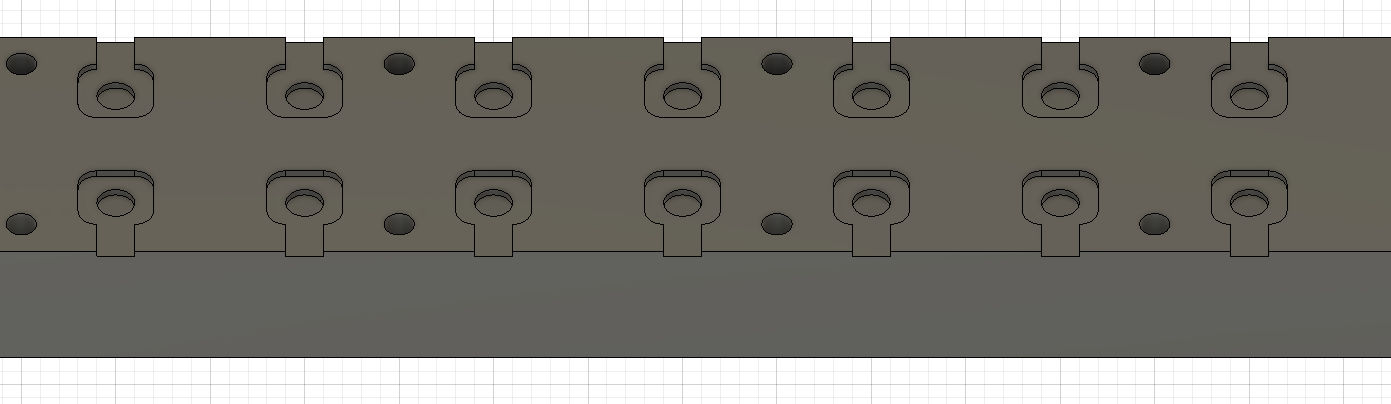
\includegraphics[width=1\textwidth]{figures/pockets.png}
    \caption{3D-model of the pockets for sensor placement}
    \label{fig:3dpockets}
\end{figure*}

The upper part of measurement block had holes of $9mm$ drilled out, for brass pistons or weight transfer pins (WTP) to be placed. As described earlier in this section, this would create a pinching effect on the sensor with the pockets. These upper brass pistons of $8.9mm$ were designed with a detachable plastic cap with threading. These rounded plastic caps were used for free movement of the ski on top of the WTP.

The side handle on the linear weight guide (can be seen in Figure \ref{fig:linearpress}) was introduced to increase ergonomic use and lower the difficulty of handling the measurement bench. The handles are placed to reduce the amount of force needed to pull the guide up for replacement of sensors and changing skis during the measurement phase.

An additional tool was designed for proper calibration of the sensors. An aluminum beam attached on the center between two supporting legs which would rest on the frame of the measurement bench (Figure \ref{fig:calibrationtool} \& Figure \ref{fig:calibrationtool_side}). At the end of the beam, a switchable loading point was attached to load individual sensors at the beam location. Weights would then be placed on top of the center of the beam, transferring the half of the loaded weight on to the sensor. When a calibration of the sensor was conducted (Section \ref{sec:calibration}), the measured values would represent the loaded weight.

\begin{figure}[!htb]
   \begin{minipage}{0.44\textwidth}
     \centering
     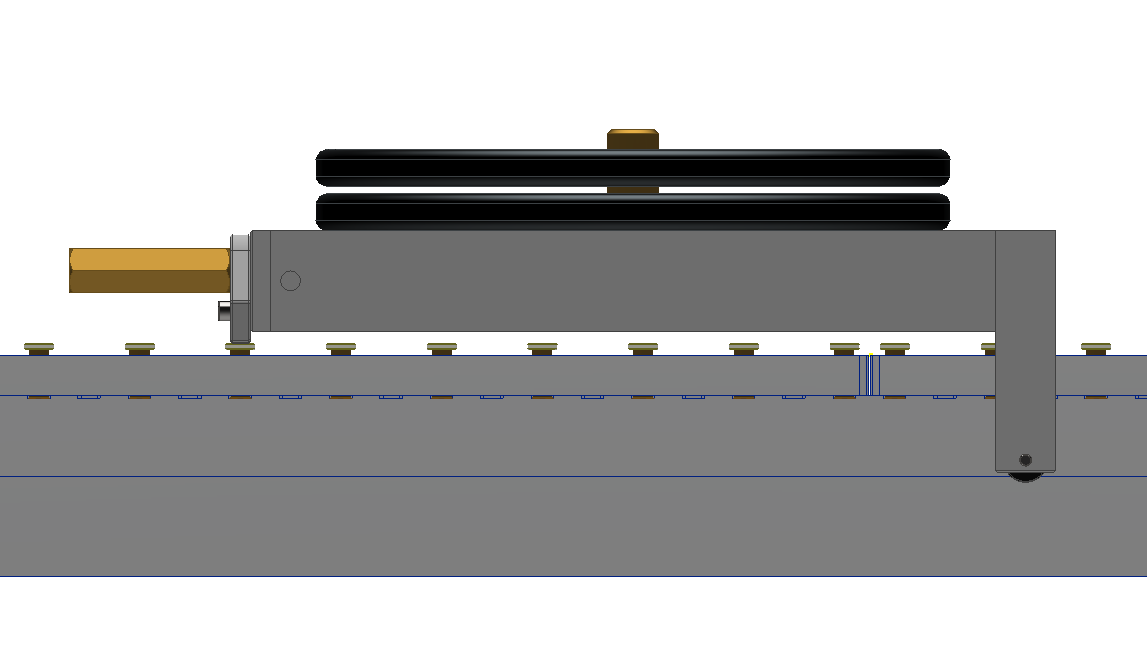
\includegraphics[width=0.9\textwidth]{figures/calibration_tool3.png}
     \caption{3D-model of the calibration tool, side view}
     \label{fig:calibrationtool}
   \end{minipage}\hfill
   \begin{minipage}{0.44\textwidth}
     \centering
     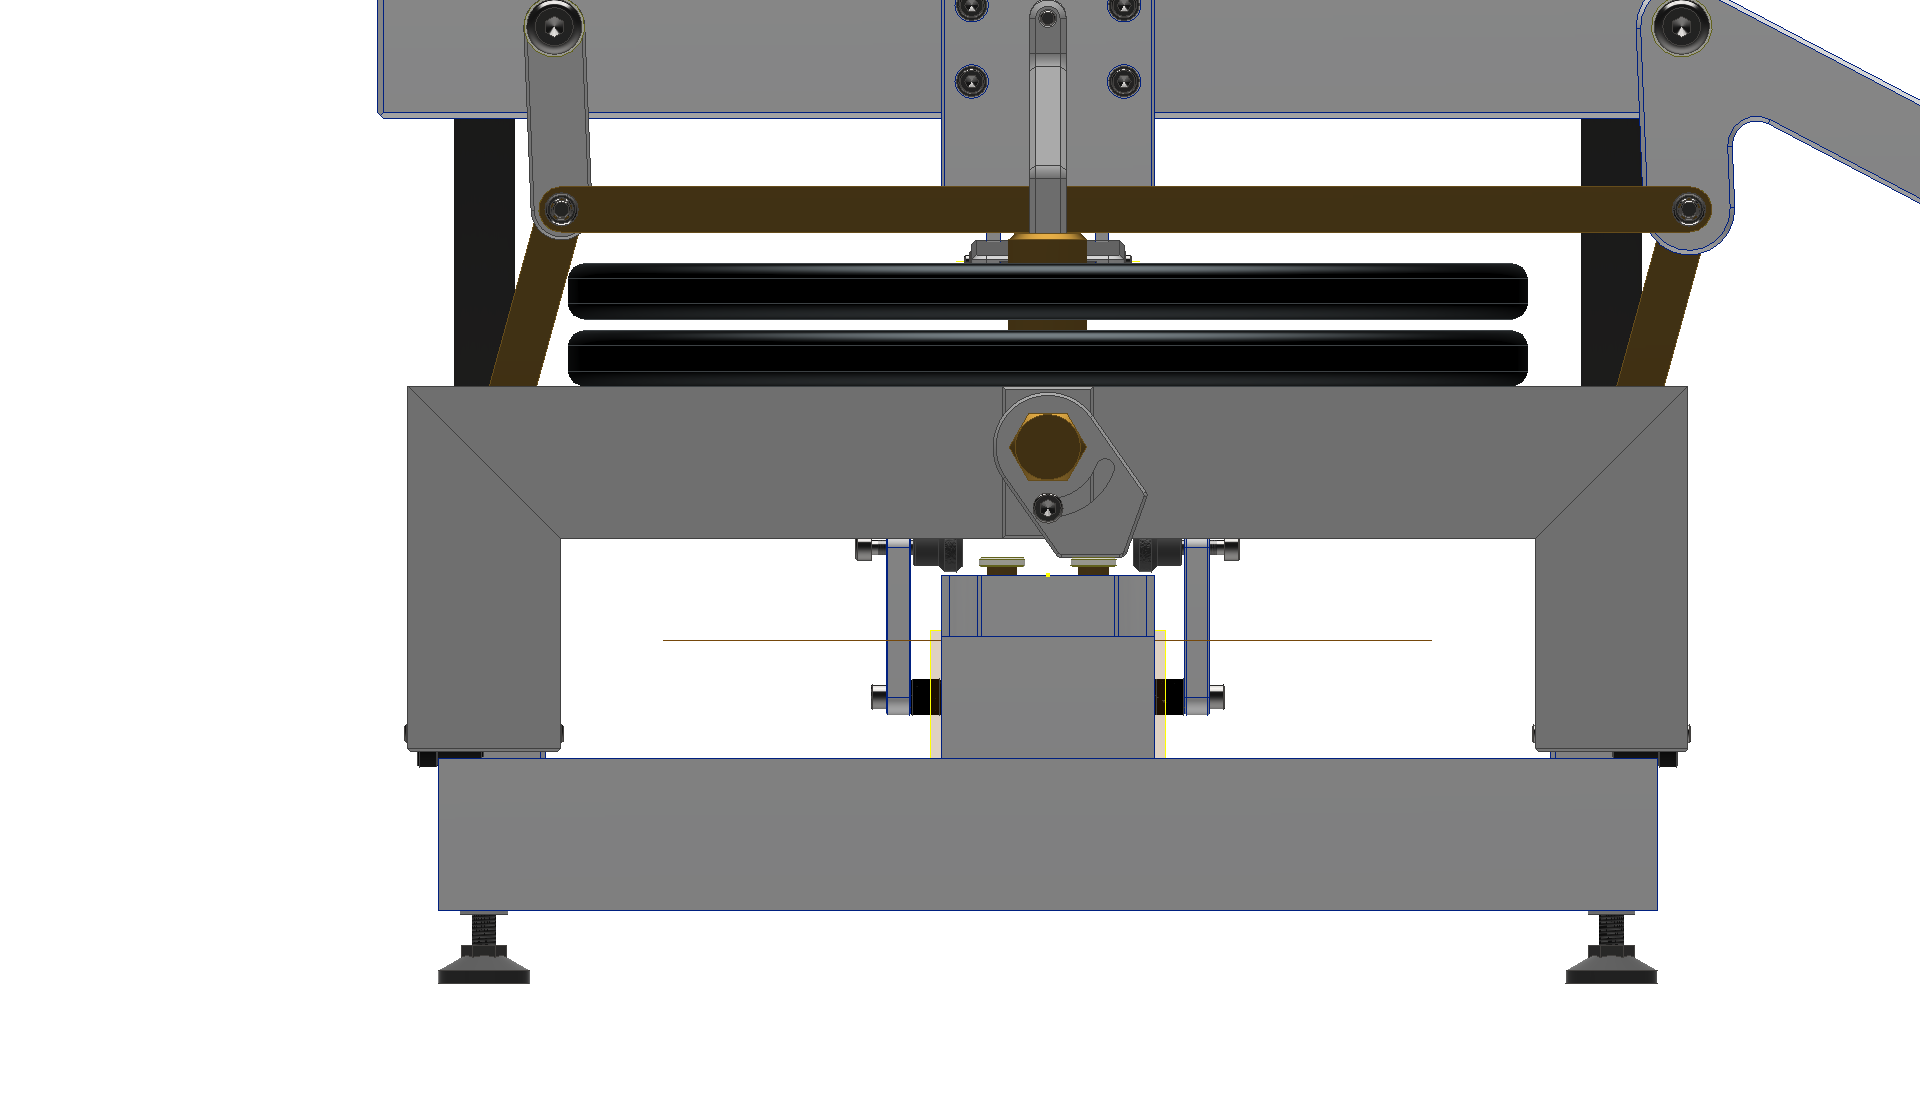
\includegraphics[width=0.9\textwidth]{figures/calibration_tool_front.png}
     \caption{3D-model of the calibration tool, front view}
     \label{fig:calibrationtool_side}
   \end{minipage}
\end{figure}

\section{The final assembly}
\label{sec:finalconcept}
The last and final concept of the measurement bench was assembled and illustrated in Figure \ref{fig:finalconcept_home} and  \ref{fig:finalconcept_side} show the final concept with all parts assembled to complete the measurement bench. The bench was manufactured and assembled by I-Lab specifically for this master thesis. After the construction and assembly, the bench was transported to the Department of Informatics for installation of sensors and the custom circuits.

\begin{figure*}
    \centering
    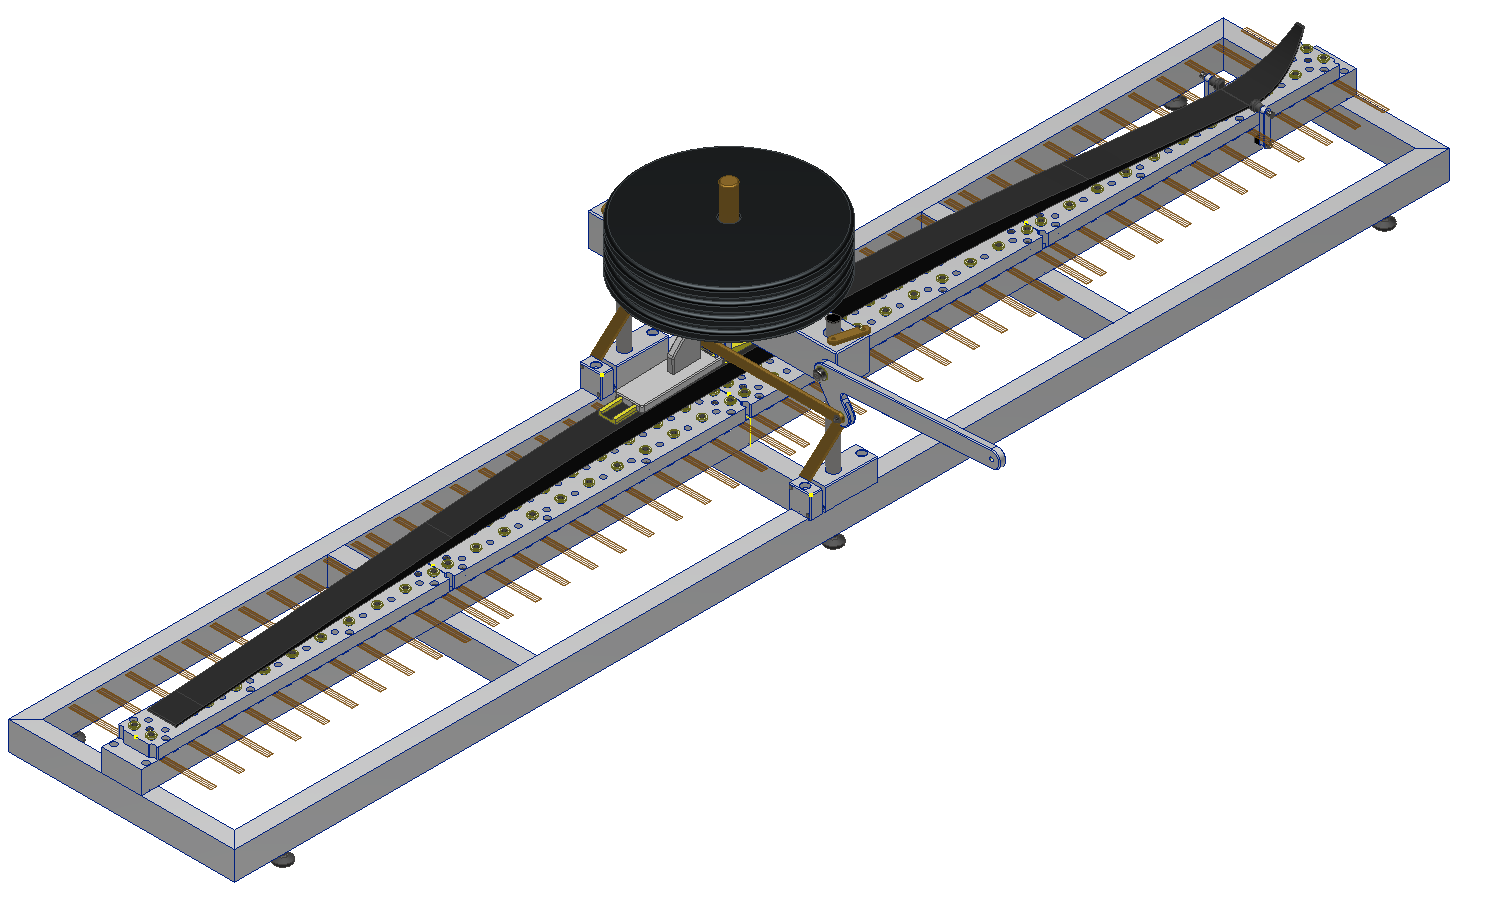
\includegraphics[width=1\textwidth]{figures/finalconcept_home3.png}
    \caption{3D-model, final concept, home view}
    \label{fig:finalconcept_home}
\end{figure*}
\begin{figure*}
    \centering
    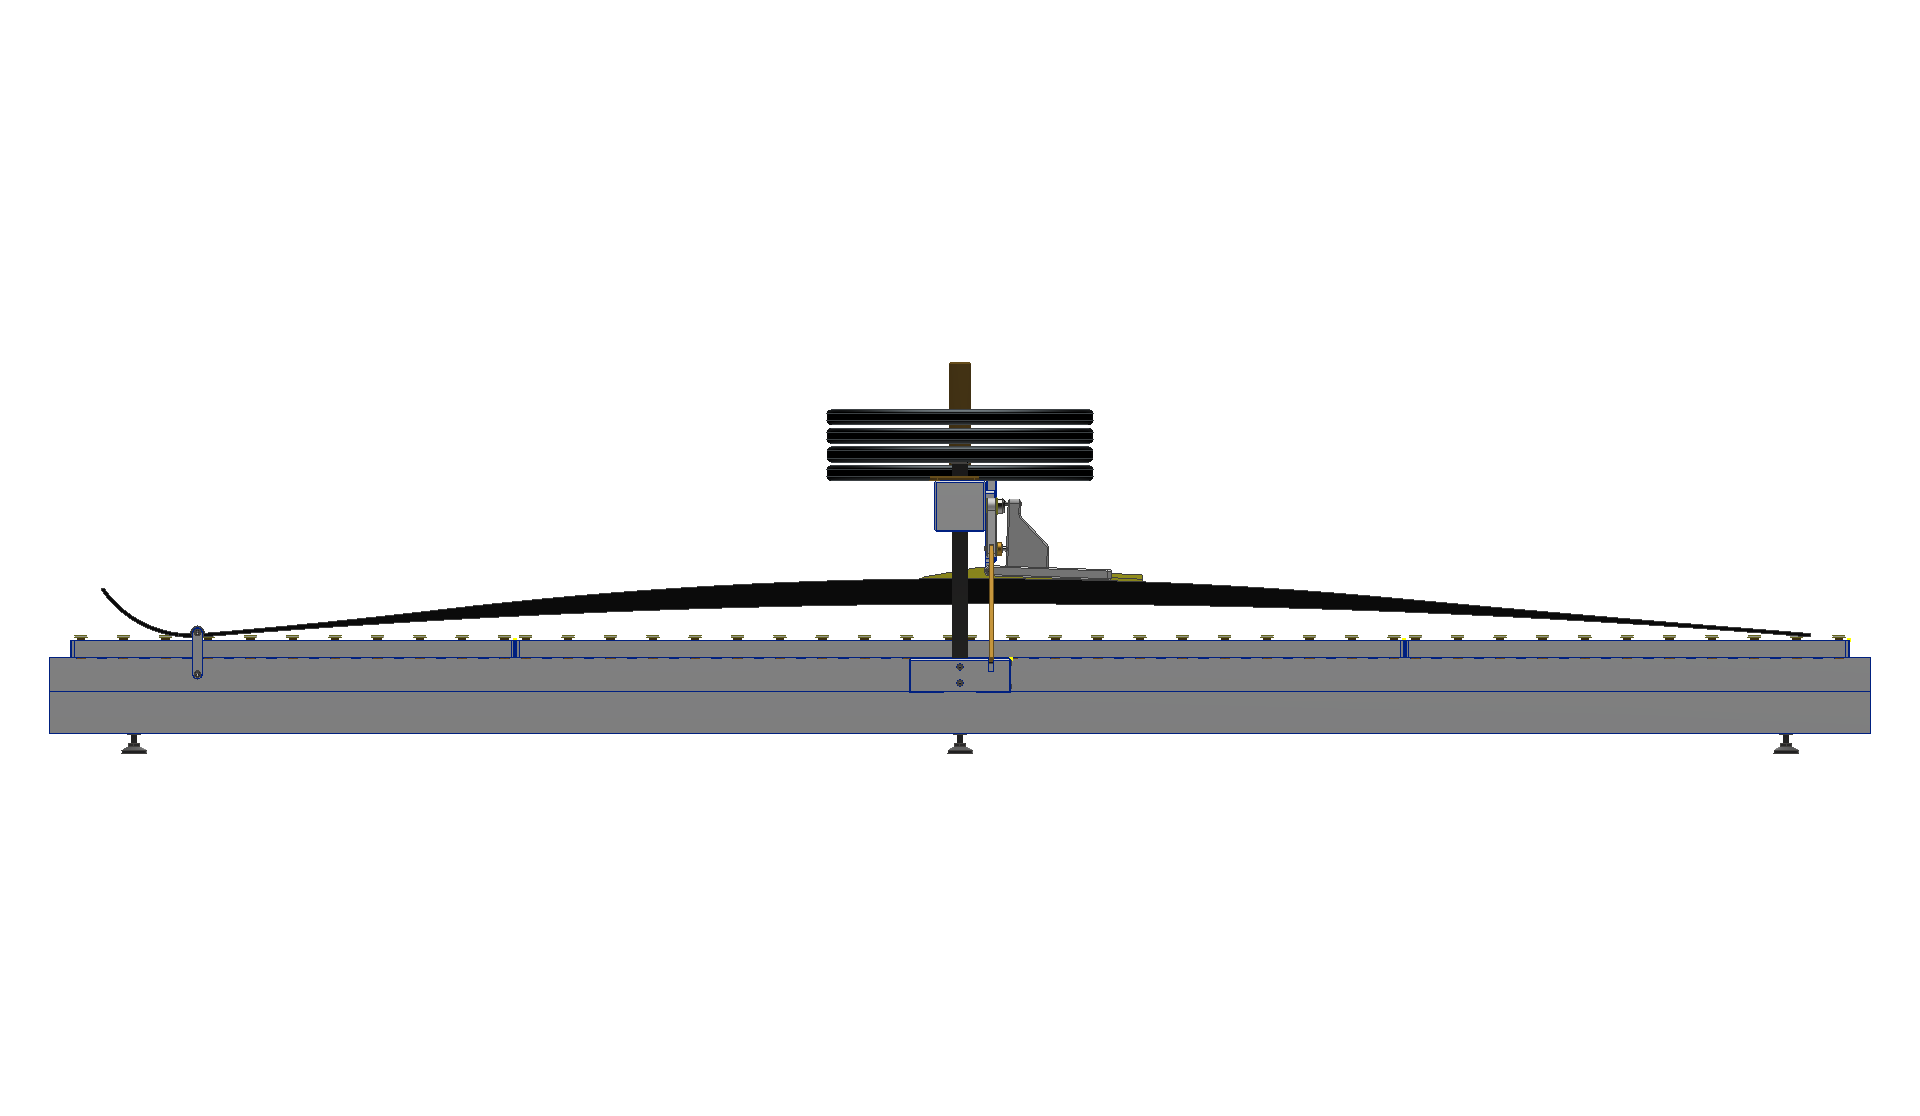
\includegraphics[width=1\textwidth]{figures/finalconcept_side.png}
    \caption{3D-model, final concept, side view}
    \label{fig:finalconcept_side}
\end{figure*}




